\chapter{Applied software and hardware}
This chapter presents the third party software and existing hardware used to create the autonomous landing system.
\section{LSTS toolchain}
The software toolchain used in the autonomous landing system was developed by the Underwater Systems and Technology Laboratory (LSTS), which is called the LSTS toolchain \citep{pinto2013lsts}. The toolchain was developed for support of networked heterogeneous air and ocean vehicle systems over wireless network. The toolchain contain four modules, namely \gls{imc}, DUNE, NEPTUS and Glued.
\subsection{IMC}
The \acrfull{imc} message protocol \citep{martins2009imc} is design to enable interconnections between systems of vehicles, sensors and human operators, which enable the pursuit of an common goal by cooperatively exchange real-time information about the environment and updated objectives. The message protocol is oriented around the message, which abstracts hardware and communication heterogeneity with a provided shared set of messages that can be serialized and transferred over different means. The \gls{imc} protocol is defined in a single eXtensible Markup Language (XML) document, which simplify the definition of exiting messages and the creation of new messages. Table \ref{Tb:IMCmessages} includes the \gls{imc} messages which is used in the \gls{uav} navigation system.
\begin{table}[H]
\centering
\begin{tabular}{| p{2.5cm} | p{9cm} |}
\hline
\textbf{Message name} & \textbf{Description} \\ \hline
EstimtedState	& Contain the current state information of the \gls{uav}, which has been made available for the DUNE system	\\ \hline
ExternalNavData & Contain the navigation data from a external navigation system	\\ \hline
NavSources		& Contain the current source of the navigation data used in the \gls{uav} navigation system, in addition to all available navigation sources\\ \hline
GpsFixRtk		& Contain the \gls{rtk-gnss} data \\ \hline
\end{tabular}
\caption{Common \gls{imc} messages used in the \gls{uav} navigation system}
\label{Tb:IMCmessages}
\end{table}
\subsection{Dune}
DUNE (DUNE Uniform Navigation Environment) is a runtime environment for unmanned systems on-board software written in C++. DUNE is capable to interact with sensors, payload and actuators, in addition to communication, navigation, control, manoeuvring, plan execution and vehicle supervision. The software separate operations into different task where each has its own thread of execution. DUNE apply a message bus which is responsible for forwarding \gls{imc} messages from the producer to all registered consumers, which is the only way different DUNE tasks is communicating. The terminology dispatch and consume is used to describe whether a task send or receive a \gls{imc} message, with dispatch is used for a sent message and consume for a received message. 

A DUNE task can be configured to be enabled in different profiles, where ArduPilot Software In the Loop (AP-SIL) and Hardware are the profiled used to test and verify the autonomous landing system. Separation is program execution profile allows for verification of a task in a simulation, where the DUNE system is executed as if it's connected to the hardware configuration.
 
\subsection{Neptus}
Neptus is a Command and Control software used to command and monitor unmanned systems. Neptus is able to provide coherent visual interface to command the vehicles in the DUNE system despite the heterogeneity in the controlled system which Netpus is interacting with. This allows the operator to command and control unmanned system without the need to dwell into specific command and control software in the unmanned system. The main communication channel for Neptus is the \gls{imc} message protocol, which makes it interoperable with DUNE or other \gls{imc}- based peer.

The Neptus console can be configured to suit an unmanned systems operational requirements by including plug-ins that express information critical to the unmanned system, in addition to plug-in used to execute certain actions from the unmanned system. This flexibility makes Neptus ideal for experimental testing of new features  applied to unmanned systems.   

Neptus can be used to review the mission logs generated by DUNE in the Mission Review and Analysis (MRA). Mission analysed in MRA can be exported to a Matlab format, which allows for a deeper analyse of the performance of a system after a completed mission.
\subsection{Glued}
Glued is a minimal Linux operating system distribution, designed with embedded system in mind. It is platform independent, easy to configure and contain only the necessary packages to run on a embedded system. This makes GLUED a light and fast distribution, which is ideal for a on-board operating system for a unmanned system where payload size is normally limited. GLUED is configured through a single configuration file that which can be created for a specific system. A advantage with Glued is that it can be cross-compiled, which allows for compilation of software before it's transferred to the embedded computer.
\section{RTKLIB}\label{ss:Rtklib}
RTKlib \citep{takasu2009development} is an open source program package for standard and precise positioning with \gls{gnss} developed by T. Takasu. RTKlib can be configured as a \gls{rtk-gnss} system, where raw \gls{gnss} data from the base station and rover is fused together, and used to estimate the relative position of the rover with respect to the base station in real time. The communication flow for a \gls{rtk-gnss} system using RTKlib in a DUNE system is shown in figure \ref{figure:RTKLIB_STRUCTURE}, where the modules str2str and rtkrcv in RTKlib is the base station software and rover software respectfully. The version of \gls{rtklib} used in this thesis is \gls{rtklib}2.4.2 \citep{Rtklib242}.

RTKlib can be configured as both a moving baseline and kinematic configuration, which is described in section \ref{ss:rtk-gps}. The configuration used in this autonomous landing system is the moving baseline configuration, due to increased operational mobility of the base station. The effect of this configuration is that the global positioning accuracy is lower then the relative position accuracy with respect to the base station. However this is not a problem for the autonomous landing system, since as long as all system participants apply gls{rtk-gnss} with the same base station position, then high baseline accuracy is good enough to safely perform a autonomous net landing. The RTKlib configuration file used in the autonomous landing system is given in appendix \ref{APPENDIX:RTKLIB}.
\begin{figure}[h]
	\centering
		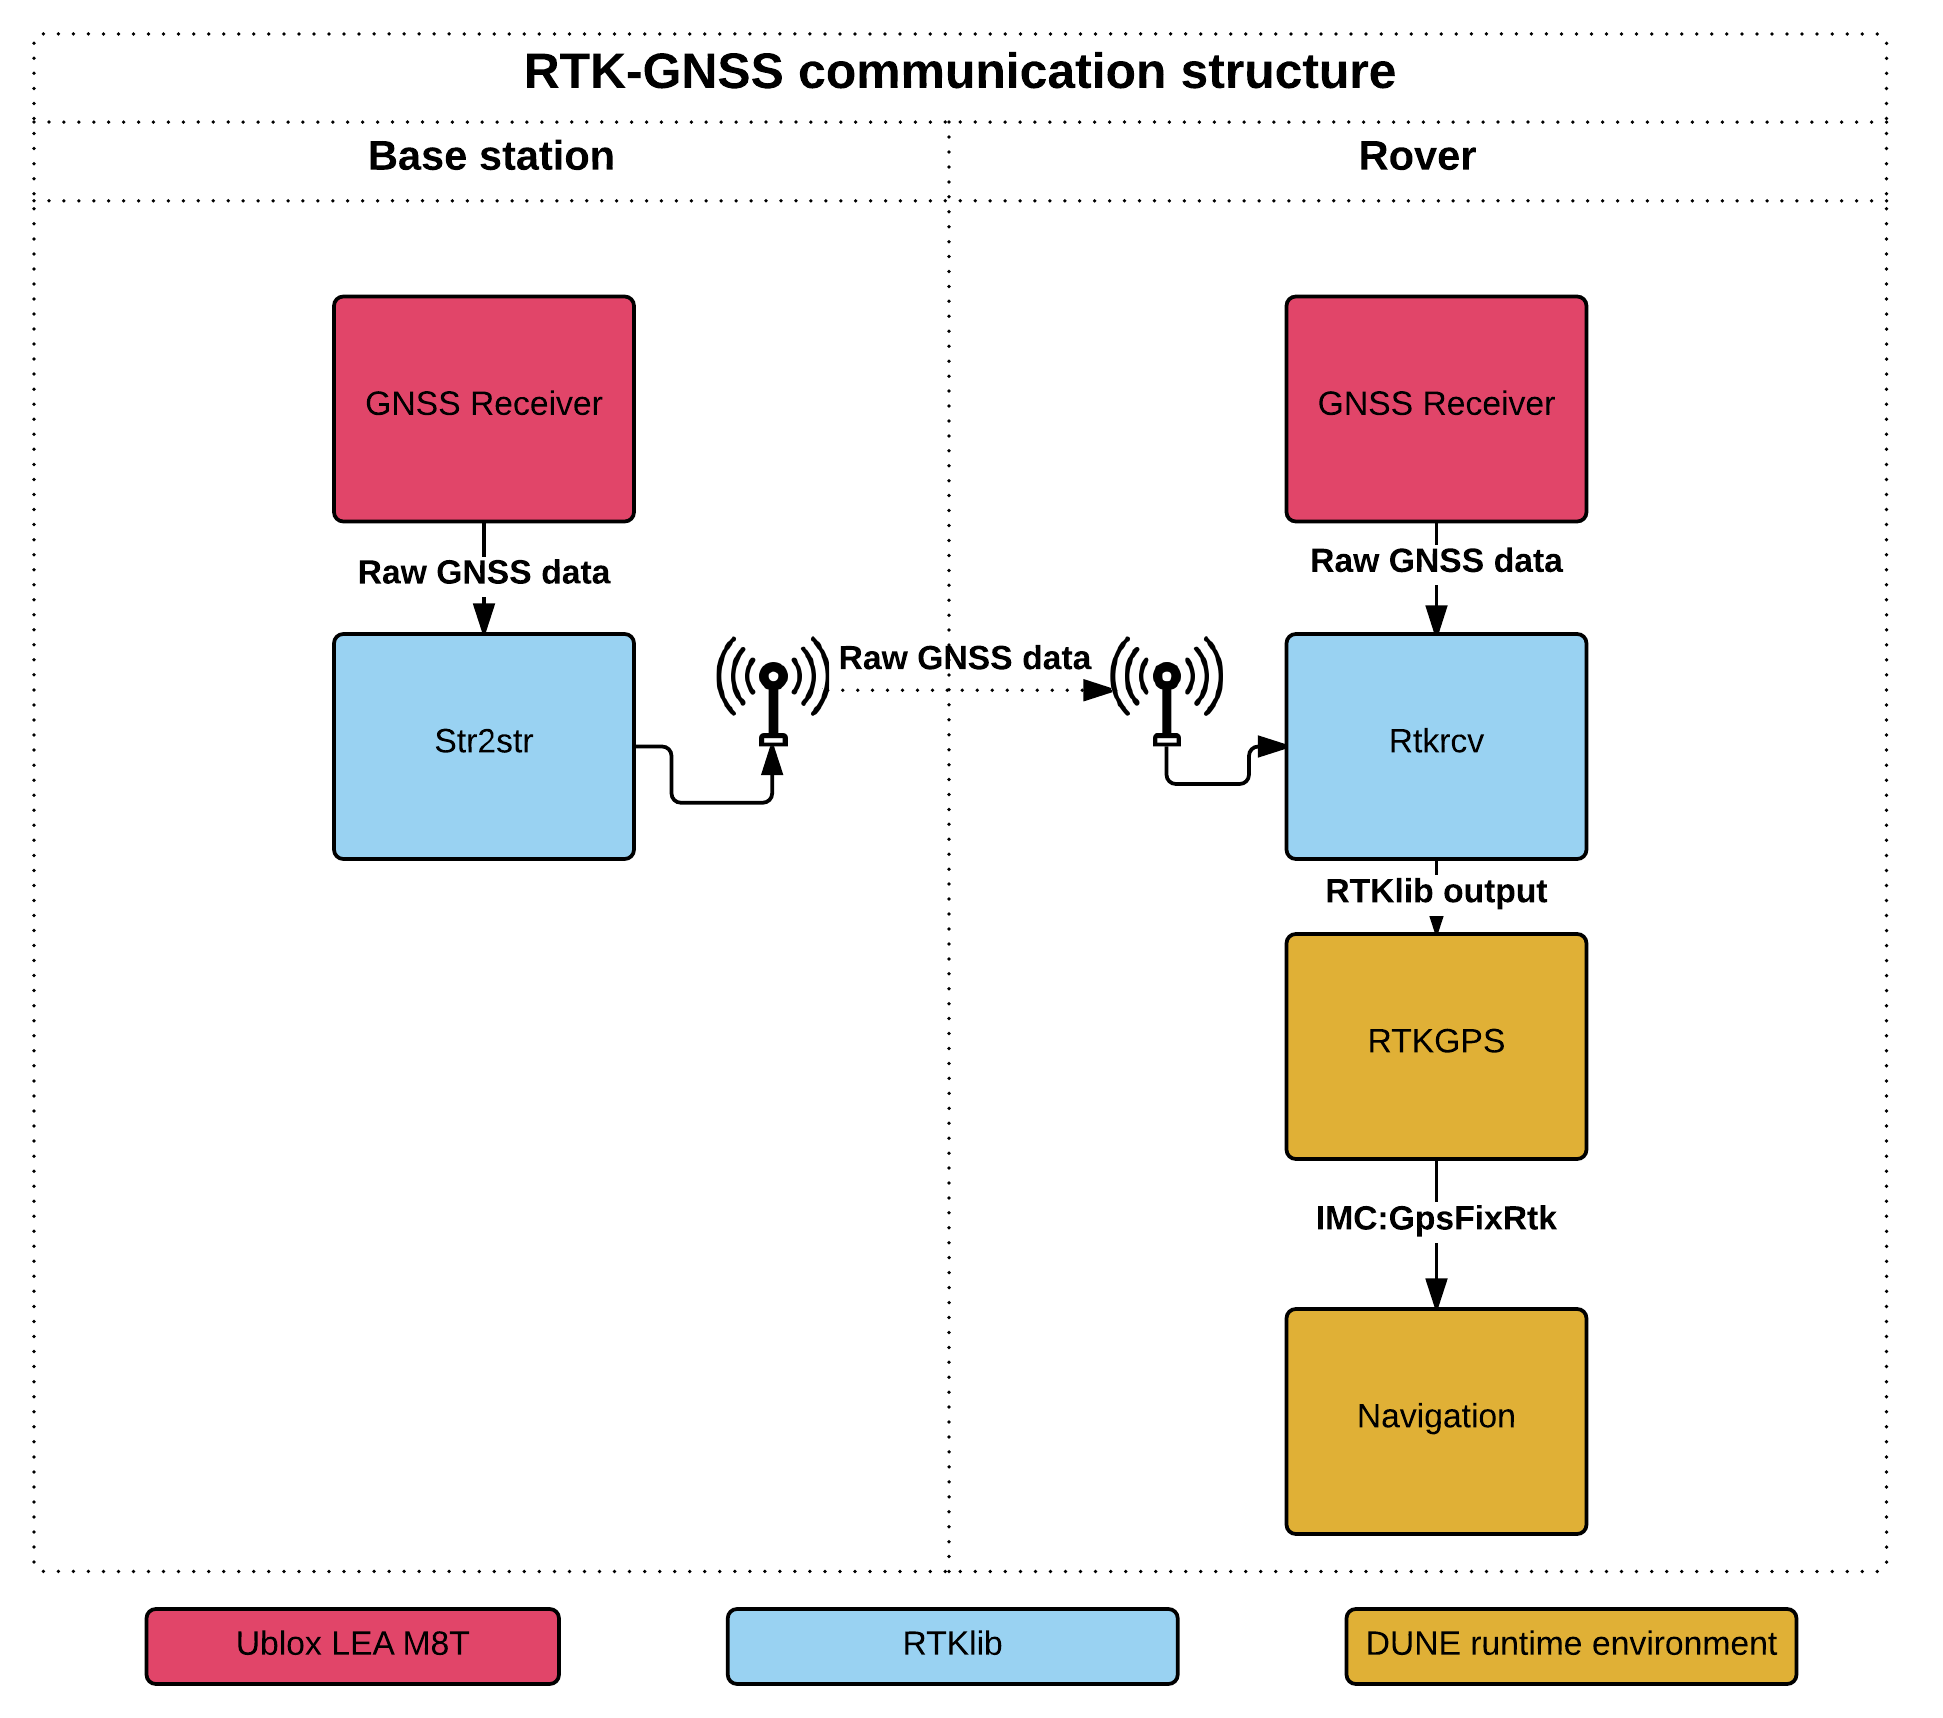
\includegraphics[scale=0.7]{figs/RTKGNSS.png}
		\caption{The communication structure a \gls{rtk-gnss} system with RTKlib, connected to DUNE}
		\label{figure:RTKLIB_STRUCTURE}
\end{figure}
\newpage

\section{Pixhawk}\label{ss:Pixhawk}
The 3DR Pixhawk is a high-performance autopilot suitable for fixed wing and multi rotors \gls{uav} and other robotic platform which can move. The Pixhawk system comes complete with \gls{gps}, imu, airspeed sensor and magnetometer, is used as an external navigation system for the DUNE environment.
\section{Ardupilot}\label{ss:ardupilot}
Ardupilot is an open-source unmanned aerial vehicle platform, able to control both fixed wing and multi rotor \glspl{uav}, and can run on the Pixhawk platform. Ardupilot allows for both manual flight control and autonomous flight operations, with a command and control software called Missionplaner. Ardupilot can be used in a Software In the Loop (SIL) simulation, where ardupilot connects to a simulator of the desired vehicle platform. This allows for verification of software before attempting a hardware test. The simulator used in a SIL simulation can be a third party software, which motivates the creation of mathematical models for the desired \gls{uav} platform. Ardupilot is used in the autonomous landing system presented in this thesis, where the low level controller is controlled in Ardupilot. The control system in Ardupilot can be separated into high and low level control. The low level control system is used in the control loops for the actuators, while the high level controller manage the desired state of the low level controllers. Ardupilot can be configured to allow for third party high level controller, which involves three levels of high level control outsourcing. The guided mode accepts way point from a third party software, however both high and low level control is managed in Ardupilot. Fly By Wire-A (FBWA) is the mode where all high level controllers are in a third party software, while Fly By Wire-B (FBWB) is a hybrid between FBWA and guided where only the lateral high level controller is in the third party software. The different mode is listen in table \ref{tb:ArduPilotMode}.
\begin{table}[H]
\centering
\begin{tabular}{| p{3cm} | p{5cm}|}
\hline
\textbf{Mode}	&	\textbf{Description} \\ \hline
Guided			& Ardupilot accept third party waypoints, and has both high and low level controllers										\\ \hline
FBWB			& Third party lateral controller with desired height controlled in a set-point regulated controller in Ardupilot \\ \hline
FBWA			& Third party lateral and longitudinal controller, with control input is sent directly to the low level controllers in Ardupilot 	\\ \hline
\end{tabular}
\caption{Guidance and control modes in autopilot viable for the landing system}
\label{tb:ArduPilotMode}
\end{table}

\section{JSBsim}
JSBSim \citep{berndt2004jsbsim} is an open-source flight dynamic model that is able to simulate a physical model of an arbitrary aircraft without the need of specific compiled and linked program code. The simulator is design such that a third party software e.g. Ardupilot can expose the model to external forces and moments. This is useful in a SITL simulator for verification of software, which is design for a hardware configuration. The physical model that was used in this thesis was developed in the master thesis \citep{Gryte}.
\section{X8 and nest payload}
The Skywalker X8 is fixed wing \gls{uav} in a flying wing configuration, which indicate that the \gls{uav} has no tail and clear distinction between the wings and fuselage. The X8 is a popular choice for experimental missions at the \gls{uav}-lab at the Deparment of Engineering Cybernetic since it's durable, cheap and enough space to carry experimental payload.

The hardware configuration used in the X8 and nest systems is based on the proposed hardware in the paper \citep{zolich2015unmanned}. The nest system is a mobile base station, which is used as both a base station and communication link between the X8 and Neptus. The X8 and the nest systems are installed with a BeagleBone embedded computer with the Glued operating system, which is used to run the Dune system, as well as RTKlib. The autopilot used in the X8 is a 3DR Pixhawk with ArduPilot ArduPlane software. For the \gls{rtk-gps} system Ublox Lea M8T GNSS receivers \citep{UbloxDataSheet,UbloxReceiverDescription} are connected to the BeagleBone with uart cable. The antenna used in the X8 is a Maxtena M1227HCT-A-SMA L1/L2 GPS-GLONASS Active Antenna \citep{maxtena}, and the antenna used in the base station is a Novatel GPS-701-GG \citep{novatel}.

The communication between the X8 and the nest systems is done with Ubiquiti M5 rocket \citep{rocketM5} radios, where the communication between each unit can be done with TCP/UDP/IP.
\cleardoublepage